% chktex-file 44
% chktex-file 1

\subsection{Analisis Kerahasiaan, Integritas, dan Ketersediaan Sistem Integrasi DecMed-PGHD}\label{analisis-cia-decmed-pghd}

Analisis pada subbab ini bertujuan menentukan persoalan keamanan dan properti yang harus dipenuhi oleh integrasi PGHD, bukan menentukan teknologi atau mekanisme implementasinya. 
Analisis mengikuti tahapan \textit{threat modelling} pada Subbab~\ref{threat-model-studi}, yaitu mengidentifikasi aset dan ruang lingkup, menentukan aktor dan batas kepercayaan secara konseptual, mengidentifikasi ancaman menggunakan STRIDE, dan memprioritaskan risiko menggunakan DREAD\@. 
Ruang lingkup analisis mencakup PGHD sejak tersedia pada sisi pasien hingga digunakan oleh tenaga kesehatan. 
Tahapan logis yang dipertimbangkan hanya meliputi perolehan, pengolahan, pengiriman, penyimpanan, dan penggunaan data. 

\subsubsection{Identifikasi Aset, Data dan Aktor}

Aset-aset yang dimiliki dan berinteraksi dengan sistem DecMed-PGHD dapat dilihat pada Tabel~\ref{tab:aset-decmed-pghd}.

\begin{table}[htb]
    \centering
    \caption{Aset pada Integrasi DecMed-PGHD}\label{tab:aset-decmed-pghd}
    \begin{styledtable}{>{\raggedright\arraybackslash}p{0.10\textwidth} >{\raggedright\arraybackslash}p{0.27\textwidth} >{\raggedright\arraybackslash}X}
        \textbf{ID} & \textbf{Aset} & \textbf{Alasan Perlindungan} \\

        A01 & Isi PGHD & Memuat informasi kesehatan dan data pasien. \\

        A02 & Metadata konteks dan \textit{provenance} & Menjelaskan pemilik, waktu, sumber, cara perolehan, dan riwayat pemrosesan data sehingga memengaruhi interpretasi serta tingkat kepercayaan terhadap PGHD\@. \\

        A03 & Identitas dan kredensial aktor & Digunakan untuk membuktikan identitas pasien maupun tenaga kesehatan dan menentukan tindakan yang boleh dilakukan. \\

        A04 & Informasi persetujuan dan hak akses & Menentukan siapa yang boleh mengakses PGHD, data milik pasien mana yang boleh diakses, tujuan atau konteks akses, masa berlaku, dan status pencabutan. \\

        A05 & Riwayat dan status data & Menjadi bukti terjadinya pengiriman, pemberian atau pencabutan akses, pemeriksaan data, serta perubahan status validitas. \\

        A06 & Keberlangsungan data dan layanan & Menjamin PGHD yang sah tidak hilang dan tetap dapat dikirim serta diakses dalam kondisi operasional. \\
    \end{styledtable}
\end{table}

Aliran data PGHD secara umum didefinisikan sebagai berikut,

\begin{enumerate}
    \item Pasien menghasilkan atau menyediakan PGHD kepada sistem.
    \item Sistem menerima, mengelola, dan mempertahankan PGHD beserta konteksnya.
    \item Pasien memberikan atau mencabut persetujuan akses.
    \item Tenaga kesehatan meminta dan menggunakan PGHD dalam konteks pelayanan.
\end{enumerate}

Hubungan antarentitas, proses, penyimpanan, dan layanan eksternal tersebut dimodelkan menggunakan DFD Level 0 dan Level 1.
DFD Level 0 pada Gambar~\ref{fig:dfd-decmed-pghd-level-0} menggambarkan diagram konteks secara keseluruhan. 
Entitas eksternal terdiri atas pasien beserta sumber PGHD, tenaga kesehatan, jaringan IOTA, IPFS, dan IOTA Gas Station. 

\begin{figure}[htbp]
    \centering
    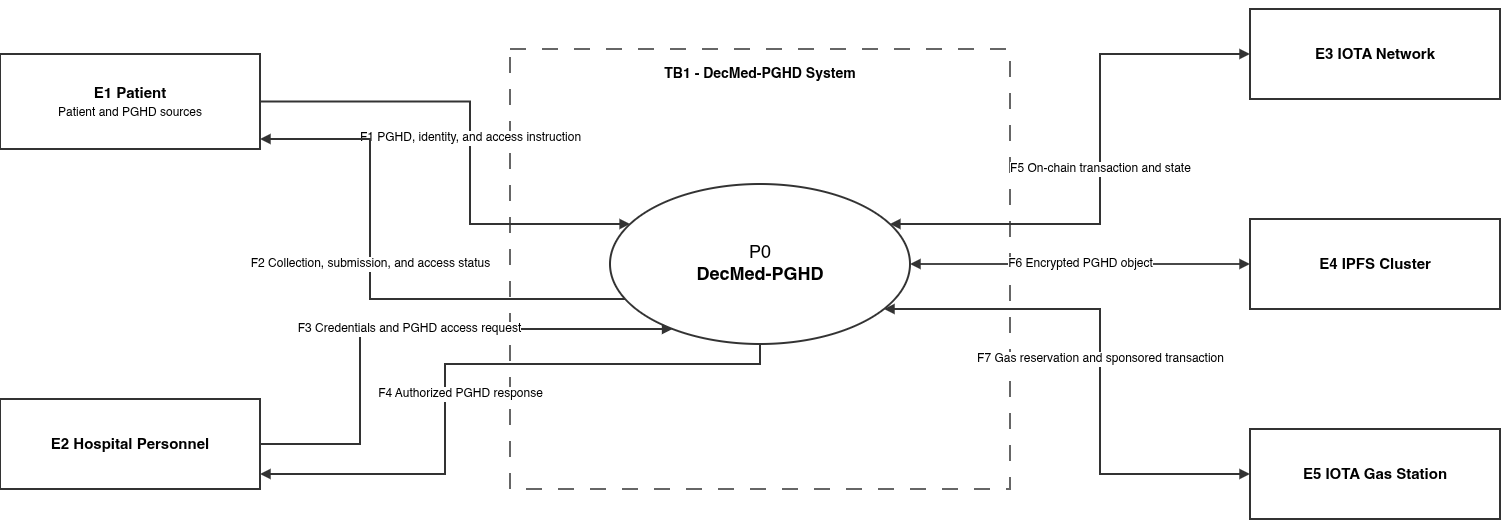
\includegraphics[width=\textwidth]{resources/chapter-3/Diagram Tugas Akhir-DFD Level 0.png}
    \caption{DFD Level 0 Sistem DecMed-PGHD untuk \textit{Threat Modelling}}\label{fig:dfd-decmed-pghd-level-0}
\end{figure}

DFD Level 1 pada Gambar~\ref{fig:dfd-decmed-pghd-level-1} menguraikan proses utama menjadi proses klien pasien, pengumpulan dan pembentukan \textit{batch}, klien tenaga kesehatan, autentikasi dan kontrol akses, penyimpanan dan pengambilan PGHD, serta \textit{proxy re-encryption} dan verifikasi. 

\begin{figure}[htbp]
    \centering
    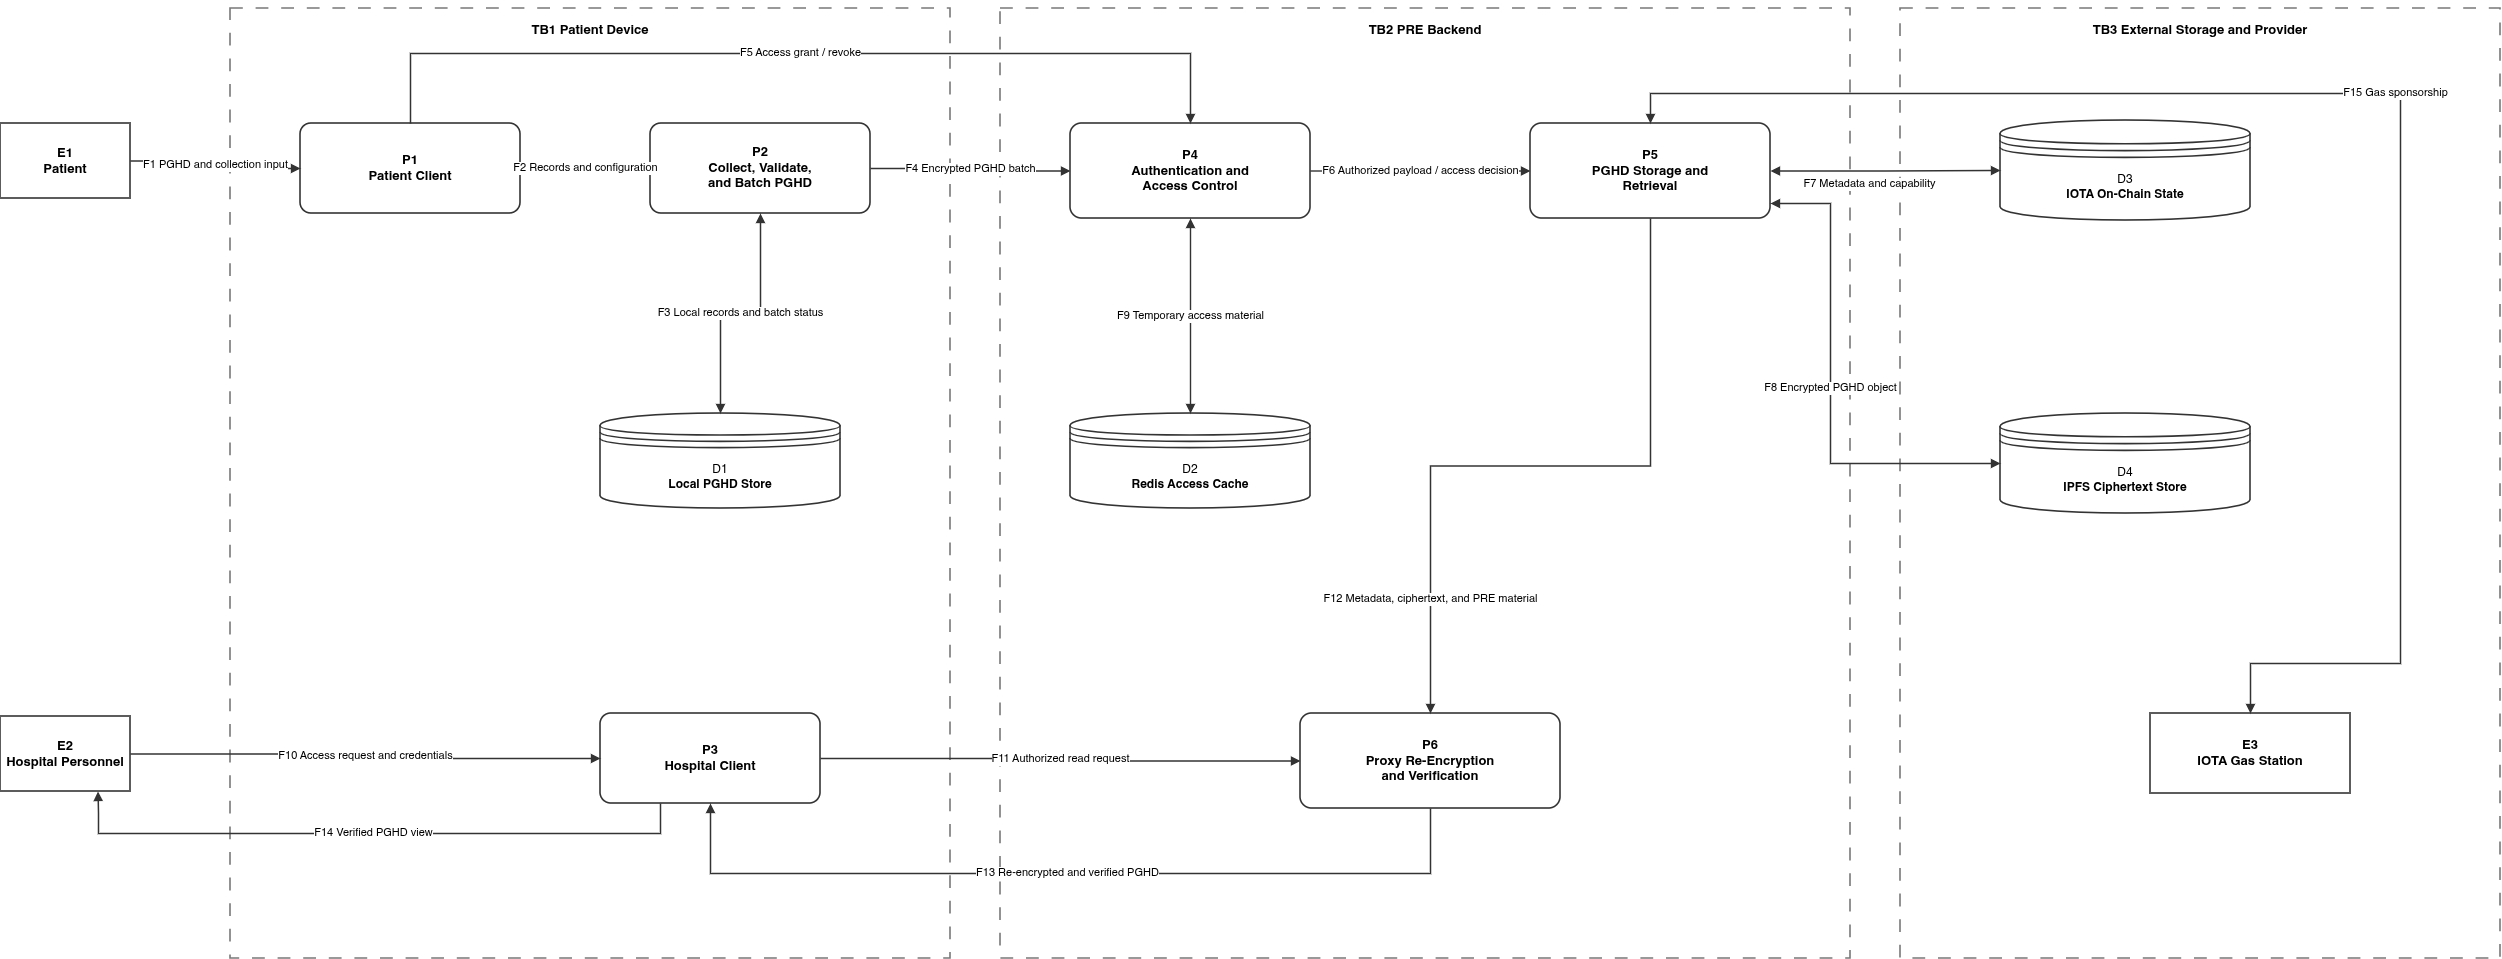
\includegraphics[width=\textwidth]{resources/chapter-3/Diagram Tugas Akhir-DFD Level 1.png}
    \caption{DFD Level 1 Sistem DecMed-PGHD untuk \textit{Threat Modelling}}\label{fig:dfd-decmed-pghd-level-1}
\end{figure}

Berdasarkan DFD tersebut, \textit{trust boundary} dipetakan terhadap komponen DecMed-PGHD seperti ditunjukkan pada Tabel~\ref{tab:trust-boundary-decmed-pghd}. 

\begin{table}[htbp]
    \centering
    \caption{Analisis \textit{Trust Boundary} DecMed-PGHD}\label{tab:trust-boundary-decmed-pghd}
    \begin{styledtable}{>{\raggedright\arraybackslash}p{0.08\textwidth} >{\raggedright\arraybackslash}p{0.18\textwidth} >{\raggedright\arraybackslash}p{0.28\textwidth} >{\raggedright\arraybackslash}X}
        \textbf{ID} & \textbf{Zona} & \textbf{Komponen} & \textbf{Risiko Utama} \\

        TB1 & \textit{Internal trusted zone} & PRE server, Redis, API \textit{backend}, konfigurasi \textit{backend} & Kebocoran kunci, penyalahgunaan material \textit{re-encryption}, manipulasi \textit{cache}, salah konfigurasi \textit{secret}, dan gangguan layanan \textit{backend}. \\

        TB2 & \textit{External untrusted zone} & \textit{Client} Android pasien, \textit{client} tenaga kesehatan, browser/desktop \textit{client}, \textit{IoT device/wearable} & Perangkat dapat hilang, terinfeksi \textit{malware}, mengirim \textit{input} tidak valid, atau digunakan untuk mencuri token. \\

        TB3 & \textit{DLT zone} & IOTA \textit{testnet}/network, \textit{smart contract public state}, transaksi \textit{on-chain} & Metadata terlihat publik, transaksi tidak dapat dihapus, biaya/gas dan ketersediaan jaringan dipengaruhi kondisi jaringan publik. \\

        TB4 & \textit{Off-chain distributed storage zone} & IPFS & \textit{Payload} terenkripsi dapat tersedia di luar kontrol langsung aplikasi; kerahasiaan bergantung pada enkripsi dan integritas bergantung pada CID/hash/signature. \\

        TB5 & \textit{Network boundary} & Komunikasi \textit{client}-PRE, PRE-IPFS, PRE-IOTA, PRE-Redis, \textit{client}-IOTA & Ancaman MITM (\textit{Man in The Middle}), penyadapan, modifikasi payload, replay, dan DoS pada endpoint. \\
    \end{styledtable}
\end{table}

Selain itu, daftar aktor atau pengguna yang memakai atau terlibat dalam sistem DecMed-PGHD ini terdapat pada Tabel~\ref{tab:aktor-trust-pghd}.

\begin{table}[htb]
    \centering
    \caption{Aktor, \textit{\textit{Privilege}}, dan \textit{\textit{Trust Level}}}\label{tab:aktor-trust-pghd}
    \begin{styledtable}{>{\raggedright\arraybackslash}p{0.20\textwidth} >{\raggedright\arraybackslash}p{0.20\textwidth} >{\raggedright\arraybackslash}X}
        \textbf{Aktor} & \textbf{\textit{Trust Level}} & \textbf{\textit{Privilege} dan Batasan} \\

        Pasien & Pemilik data yang perlu diautentikasi & Menyediakan PGHD dan mengatur persetujuan akses atas data miliknya. \\

        Tenaga kesehatan & Pengguna profesional yang perlu diautentikasi dan diotorisasi & Membaca PGHD setelah disetujui pasien. \\

        Sumber atau aplikasi penghasil PGHD & Kepercayaan terbatas & Menghasilkan nilai dan informasi konteks PGHD\@. \\

        Layanan eksternal & Kepercayaan terbatas & Dapat menyediakan layanan komunikasi, komputasi, dan penyimpanan, tetapi tidak boleh diasumsikan bebas dari kegagalan, kebocoran, atau penyalahgunaan. \\

        Penyerang eksternal atau lokal & Tidak tepercaya & Dapat mengirim \textit{input} berbahaya, mengamati komunikasi, memperoleh data sensitif, memodifikasi data, atau mengganggu layanan. \\
    \end{styledtable}
\end{table}

\subsubsection{Identifikasi Ancaman STRIDE}

Ancaman diidentifikasi dengan menerapkan STRIDE pada entitas, proses, data store, dan aliran dalam Gambar~\ref{fig:dfd-decmed-pghd-level-0} dan Gambar~\ref{fig:dfd-decmed-pghd-level-1}. 
Sesuai ruang lingkup analisis CIA, kategori ancaman yang digunakan adalah \textit{Tampering}, \textit{Information Disclosure}, dan \textit{Denial of Service}.
Ancaman-ancaman yang diidentifikasi dapat dilihat pada Tabel~\ref{tab:stride-threat-analysis-decmed-pghd}.

\begingroup
\footnotesize
\begin{styledxltabular}{|>{\raggedright\arraybackslash}p{0.06\textwidth}|>{\raggedright\arraybackslash}p{0.19\textwidth}|>{\raggedright\arraybackslash}p{0.19\textwidth}|>{\raggedright\arraybackslash}p{0.11\textwidth}|>{\raggedright\arraybackslash}X|}
\hiderowcolors
\caption{Ancaman STRIDE DecMed-PGHD}\label{tab:stride-threat-analysis-decmed-pghd}\\
\hline
\rowcolor{headerBg}
\textbf{ID} & \textbf{Ancaman} & \textbf{Aset dan Tahap} & \textbf{\textit{Trust Boundary}} & \textbf{Deskripsi} \\
\hline
\showrowcolors
\endfirsthead

\hiderowcolors
\caption[]{Ancaman STRIDE DecMed-PGHD (lanjutan)}\\
\hline
\rowcolor{headerBg}
\textbf{ID} & \textbf{Ancaman} & \textbf{Aset dan Tahap} & \textbf{\textit{Trust Boundary}} & \textbf{Deskripsi} \\
\hline
\showrowcolors
\endhead

T-T01 & Modifikasi data selama perpindahan atau penyimpanan & A01, A02, A05; pengiriman dan penyimpanan & TB1, TB4, TB5 & Isi atau metadata PGHD diubah tanpa hak dan perubahan tersebut tidak terdeteksi sebelum data digunakan. \\
\hline
T-T02 & Manipulasi persetujuan, hak akses, atau status data & A04, A05; penyimpanan dan penggunaan & TB1, TB3, TB5 & Cakupan, masa berlaku, pencabutan akses, atau status validitas diubah tanpa kewenangan. \\
\hline
T-I01 & Akses PGHD tanpa persetujuan yang sah & A01--A04; penggunaan & TB1, TB2, TB5 & Pihak yang tidak berhak memperoleh isi PGHD atau informasi sensitif yang dapat digunakan untuk membukanya. \\
\hline
T-I02 & Kebocoran data selama pengolahan, pengiriman, atau penyimpanan & A01--A03; siklus data & TB1, TB4, TB5 & Isi PGHD atau metadata sensitif dapat diamati oleh komponen, layanan, atau pihak yang tidak memerlukannya. \\
\hline
T-D01 & Volume atau frekuensi PGHD melebihi kemampuan sistem & A06; perolehan hingga penyimpanan & TB1, TB2, TB4 & Pertumbuhan data membuat proses pengumpulan, pengiriman, atau penyimpanan gagal atau mengalami degradasi yang tidak dapat diterima. \\
\hline
T-D02 & Gangguan konektivitas atau dependensi layanan & A06; lintas tahap & TB1, TB3, TB4, TB5 & Data yang sah hilang, tertunda tanpa status jelas, atau tidak dapat diakses ketika koneksi maupun layanan pendukung gagal sementara. \\
\hline
\end{styledxltabular}
\endgroup

Setiap parameter DREAD diberi nilai 1~-~10. 
Total 35~-~50 dikategorikan tinggi, 20~-~34 sedang, dan di bawah 20 rendah. 
Tabel penilaian DREAD terhadap ancaman yang diidentifikasi pada Tabel~\ref{tab:stride-threat-analysis-decmed-pghd} dapat dilihat pada Tabel~\ref{tab:dread-scoring-decmed-pghd}.

\begin{styledxltabular}{|>{\raggedright\arraybackslash}p{0.10\textwidth}|>{\centering\arraybackslash}p{0.07\textwidth}|>{\centering\arraybackslash}p{0.07\textwidth}|>{\centering\arraybackslash}p{0.07\textwidth}|>{\centering\arraybackslash}p{0.07\textwidth}|>{\centering\arraybackslash}p{0.07\textwidth}|>{\centering\arraybackslash}p{0.09\textwidth}|>{\raggedright\arraybackslash}X|}
\hiderowcolors
\caption{Penilaian DREAD Ancaman DecMed-PGHD}\label{tab:dread-scoring-decmed-pghd}\\
\hline
\rowcolor{headerBg}
\textbf{ID} & \textbf{D} & \textbf{R} & \textbf{E} & \textbf{A} & \textbf{Di} & \textbf{Total} & \textbf{Prioritas} \\
\hline
\showrowcolors
\endfirsthead

\hiderowcolors
\caption[]{Penilaian DREAD Ancaman DecMed-PGHD (lanjutan)}\\
\hline
\rowcolor{headerBg}
\textbf{ID} & \textbf{D} & \textbf{R} & \textbf{E} & \textbf{A} & \textbf{Di} & \textbf{Total} & \textbf{Prioritas} \\
\hline
\showrowcolors
\endhead

T-I01 & 10 & 8 & 7 & 8 & 8 & 41 & Tinggi \\
\hline
T-I02 & 10 & 8 & 7 & 8 & 8 & 41 & Tinggi \\
\hline
T-T02 & 9 & 8 & 7 & 8 & 8 & 40 & Tinggi \\
\hline
T-T01 & 9 & 8 & 7 & 8 & 7 & 39 & Tinggi \\
\hline
T-D02 & 8 & 8 & 7 & 7 & 7 & 37 & Tinggi \\
\hline
T-D01 & 7 & 8 & 7 & 7 & 6 & 35 & Tinggi \\
\hline
\end{styledxltabular}

\textit{Damage potential} (D) menilai kerugian terhadap kerahasiaan, integritas, dan keberlangsungan layanan.
\textit{Reproducibility} (R) menilai kemudahan serangan diulangi terhadap data atau pengguna lain setelah jalur serangan diketahui.
\textit{Exploitability} (E) menilai kebutuhan akses, kemampuan teknis, dan material khusus untuk menjalankan serangan.
\textit{Affected users} (A) menilai luas pasien, tenaga kesehatan, atau komponen yang terdampak.
\textit{Discoverability} (Di) menilai kemudahan menemukan permukaan serangan dari antarmuka, metadata publik, dan perilaku sistem.
Dasar penentuan nilai DREAD untuk setiap ancaman adalah sebagai berikut.

\begin{itemize}
    \item \textbf{T-I01 dan T-I02 memperoleh 41 (tinggi).}
    Kebocoran PGHD menimbulkan dampak privasi terbesar sehingga \textit{damage potential} bernilai 10.
    Jalur akses dan penyimpanan digunakan berulang oleh banyak data, menyebabkan \textit{reproducibility}, \textit{affected users}, dan \textit{discoverability} bernilai 8.
    \textit{Exploitability} bernilai 7 karena penyerang masih memerlukan posisi pada komponen, jaringan, penyimpanan, atau kredensial yang relevan.

    \item \textbf{T-T02 memperoleh 40 (tinggi).}
    Manipulasi persetujuan dapat membuka akses tidak sah atau mempertahankan akses yang seharusnya dicabut, sehingga \textit{damage potential} bernilai 9.
    Data persetujuan digunakan pada setiap pemeriksaan akses dan antarmuka pengelolaannya dapat diamati, sehingga \textit{reproducibility}, \textit{affected users}, dan \textit{discoverability} bernilai 8.
    \textit{Exploitability} bernilai 7 karena perubahan tetap membutuhkan akses ke jalur transaksi, state, atau komponen otorisasi.

    \item \textbf{T-T01 memperoleh 39 (tinggi).}
    Perubahan pada \textit{ciphertext}, metadata, CID, atau status dapat menyebabkan data salah digunakan atau tidak dapat dibuka, sehingga \textit{damage potential} bernilai 9.
    Titik perpindahan dan penyimpanan dilalui semua \textit{batch} dan memungkinkan serangan diulang, sehingga \textit{reproducibility} dan \textit{affected users} bernilai 8.
    \textit{Exploitability} dan \textit{discoverability} bernilai 7 karena penyerang harus mencapai jaringan, PRE, IPFS, atau metadata terkait.

    \item \textbf{T-D02 memperoleh 37 (tinggi).}
    Ketergantungan pada konektivitas, PRE, IPFS, IOTA, dan layanan pendukung membuat gangguan sementara berdampak pada alur lintas tahap, sehingga \textit{damage potential} dan \textit{reproducibility} bernilai 8.
    \textit{Exploitability}, \textit{affected users}, dan \textit{discoverability} bernilai 7 karena gangguan dapat dipicu atau terjadi pada beberapa dependensi, tetapi tidak selalu memengaruhi seluruh pengguna secara permanen.

    \item \textbf{T-D01 memperoleh 35 (tinggi).}
    PGHD berbentuk \textit{time-series} dan dapat tumbuh cepat, sehingga serangan atau beban berlebih mudah diulang (\textit{reproducibility} bernilai 8).
    \textit{Damage potential}, \textit{exploitability}, dan \textit{affected users} bernilai 7 karena kelebihan beban dapat menghentikan pengiriman dan penyimpanan pada banyak batch, sedangkan \textit{discoverability} bernilai 6 karena batas kapasitas aktual baru terlihat setelah pengujian beban.
\end{itemize}

Seluruh ancaman berprioritas tinggi dipilih sebagai dasar kebutuhan non-fungsional. 
